\documentclass[tikz,border=5mm]{standalone}
\usepackage{amsmath}
\usetikzlibrary{automata, positioning, arrows.meta, backgrounds}
\begin{document}
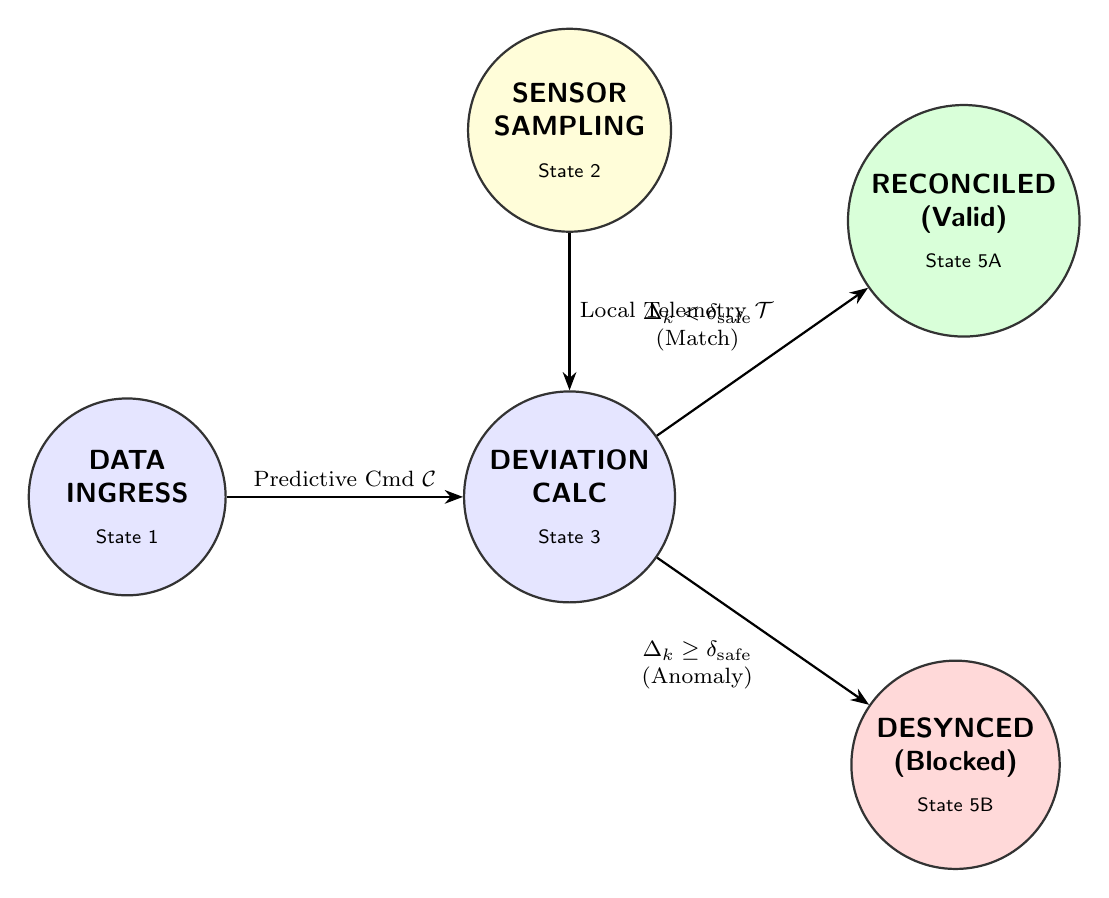
\begin{tikzpicture}[
    font=\sffamily,
    ->, >=Stealth, thick,
    node distance=3cm,
    state/.style={circle, draw=black!80, fill=blue!10, thick, minimum size=2.5cm, align=center}
]

\node[state] (ingress) {\textbf{DATA}\\\textbf{INGRESS}\\[1mm]\scriptsize State 1};
\node[state, right=3cm of ingress] (dev) {\textbf{DEVIATION}\\\textbf{CALC}\\[1mm]\scriptsize State 3};
\node[state, fill=green!15, above right=1.5cm and 3cm of dev] (valid) {\textbf{RECONCILED}\\\textbf{(Valid)}\\[1mm]\scriptsize State 5A};
\node[state, fill=red!15, below right=1.5cm and 3cm of dev] (blocked) {\textbf{DESYNCED}\\\textbf{(Blocked)}\\[1mm]\scriptsize State 5B};
\node[state, fill=yellow!15, above=2cm of dev] (sensor) {\textbf{SENSOR}\\\textbf{SAMPLING}\\[1mm]\scriptsize State 2};

\path 
    (ingress) edge node[above, font=\footnotesize] {Predictive Cmd $\mathcal{C}$} (dev)
    (sensor) edge node[right, font=\footnotesize] {Local Telemetry $\mathcal{T}$} (dev)
    (dev) edge node[above left, font=\footnotesize, align=center] {$\Delta_k < \delta_{\text{safe}}$\\(Match)} (valid)
    (dev) edge node[below left, font=\footnotesize, align=center] {$\Delta_k \ge \delta_{\text{safe}}$\\(Anomaly)} (blocked);

\end{tikzpicture}
\end{document}
